\section{Results \& Discussion}
% aggregation of a random value from 0 to 1000
As showed in Figure \ref{fig: result}, for each topology, state of every node in every epoch is plotted. Inside 100 epochs all four experiments are in the trend of converging and if we set convergence criteria as 5\% of mean value, Bren, Geant and Iij can be considered as converged inside their run of experiments, accordingly at 75th, 60th and 40th epoch.\\
Thus, the order of convergence speed can be derived as Iij, Geant, Bren, Reuna, from the fastest to slowest, which verifies our hypothesis.
\begin{figure}[h!]
	\centering
    \begin{minipage}[t]{0.47\textwidth}
    \vspace{0pt}
    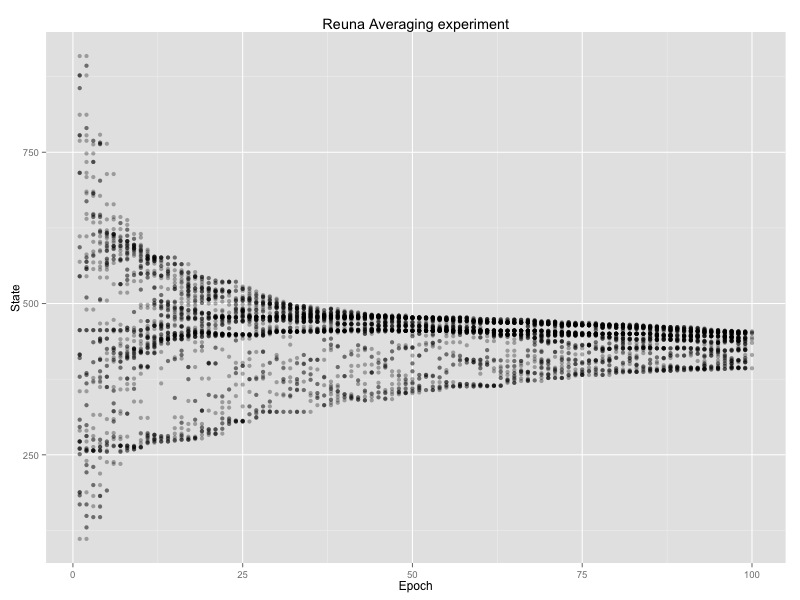
\includegraphics[width=\linewidth]{figures/Reuna.png}
    Reuna Averaging experiment
    \end{minipage}
    %\vspace{5ex}
    \begin{minipage}[t]{0.47\textwidth}
    \vspace{0pt}
    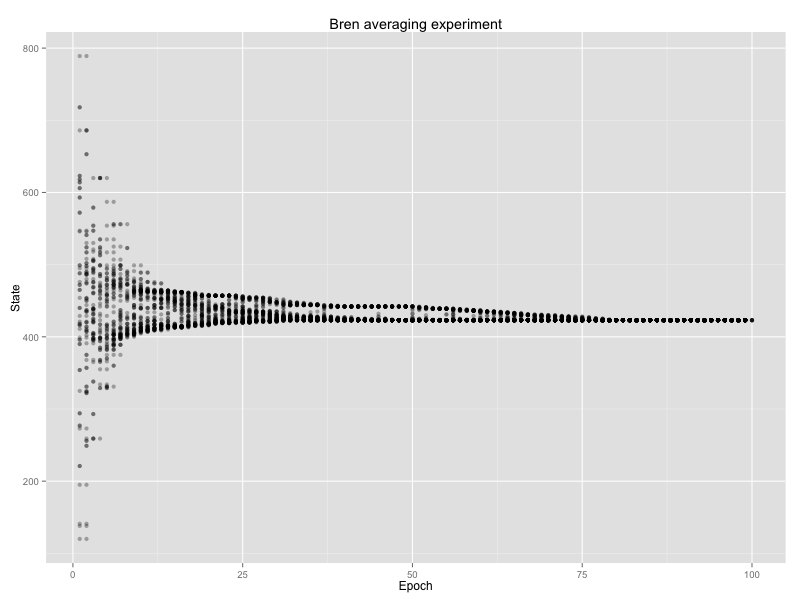
\includegraphics[width=\linewidth]{figures/Bren.png}
    Bren Averaging experiment
    \end{minipage}
    \vspace{5ex}
    \begin{minipage}[t]{0.47\textwidth}
    \vspace{0pt}
    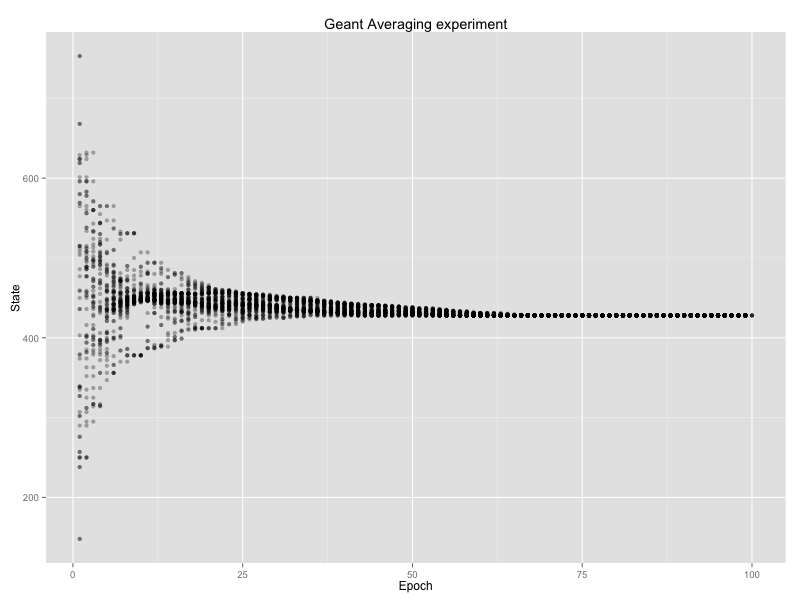
\includegraphics[width=\linewidth]{figures/Geant.png}
    Geant Averaging experiment
    \end{minipage}
    %\vspace{5ex}
    \begin{minipage}[t]{0.47\textwidth}
    \vspace{0pt}
    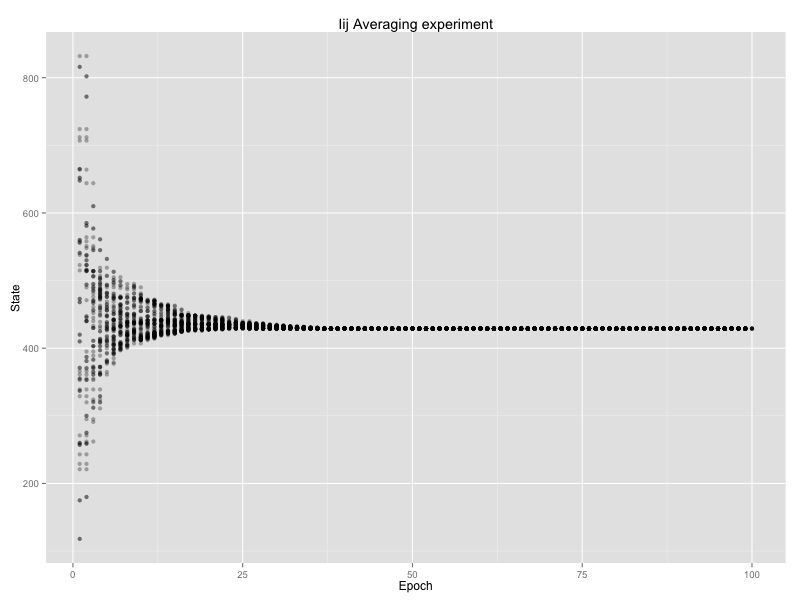
\includegraphics[width=\linewidth]{figures/Iij.png}
    Iij averaging experiment
    \end{minipage}
    \caption{}
    \label{fig: result}
\end{figure}


% explain the graphs
% Draw a conclusion about the difference
% compare emulation and simulation

\begin{figure}[h!]
    \begin{center}
    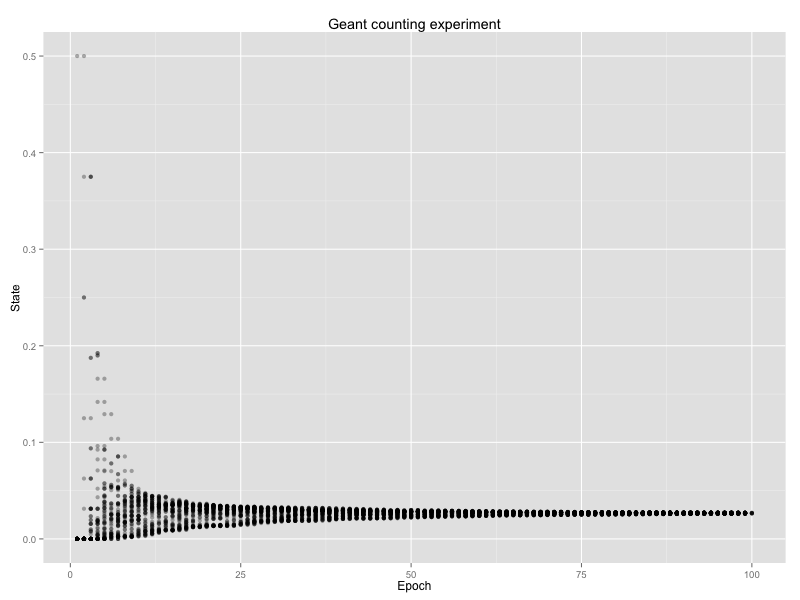
\includegraphics[width=\linewidth]{figures/geant_counting_exp.png}
    \end{center}
    \caption{Geant counting}
    \label{fig:geant}
\end{figure}
\label{sec:results}
